\documentclass{article}

\usepackage{graphicx}
\usepackage{hyperref}
\usepackage{amssymb}

\title{Yelp and Crime}  % TODO
\author{Kenneth Lin, Sid Naik, Tom McCormick}
\date{\today}

\providecommand{\e}[1]{\ensuremath{\times 10^{#1}}}

\renewcommand{\labelitemi}{\checkmark}

\begin{document}
\maketitle

\section{Problem Statement and Background}

For our CS 194 final project, we decided to investigate the potential
relationship between the City of San Francisco public safety data set and
the data set provided by the Yelp API. With the recent civil unrest both
inside and outside of the United States, and more recently, right here in
Berkeley, we thought that it would be interesting to look into the factors
that promote crime. One of our team members (Kenneth Lin) had also been
robbed recently, so the problem is one that is dear to our hearts. Perhaps
the most well-known correlation with crime rate is the income level of a
neighborhood -- the lower the income level, the higher the crime rate
\cite[p.93-94]{levitt-the-changing-relationship}. However, we wanted to
show something more interesting. In particular, Yelp restaurants, in our
experience, often reflect the wealth and well-being of its surrounding
neighborhood -- the presence of many highly rated restaurants, we believed,
reflect the optimism in the economy of a neighborhood, as well as the
wealth and ``goodness'' of that neighborhood. Therefore, we had conjectured
that crime would negatively impact restaurant ratings, or that low
restaurant ratings would be correlated with areas of high crime. We worked
to show this throughout our project.

% At first, we explored each data set individually to discover general
% patterns in the data set. After that, we delved into our main problem. We
% are interested in the relationship (if any) between the quality of
% restaurants and the frequency and severity of crime. In particular, we
% wanted to know

In particular, we wanted to know
\begin{itemize}
\item the effect of crime on restaurant ratings (or vice versa)
\item the distribution of crime vs. the distribution of ratings
\end{itemize}

We had also wanted to predict crime density / severity using restaurant
ratings or vice versa, but along the way we ran into issues of determining
or implying causation in any of the methods we used. By using one to
predict the other and trying to draw useful conclusions from this, we run
the risk of assuming causation without definitive proof. There are many
other problems that may arise as a result of this, which will be discussed
in the \textbf{\nameref{sec:lessons-learned}} section.

\subsection{City of San Francisco Public Safety Data Set}

The City of San Francisco public safety data set is a record, written by
the San Francisco Police Department, of incoming incident reports, either
via phone call, in person, or otherwise. These incidents, reported via the
SFPD CABLE crime incident reporting system, cover the span of more than 11
years, from 1/1/2003 to present. Incidents are recorded when a police
report is filled out during or after a crime incident. Crimes range from
aggravated assault to vandalism to death reports.

A sample of records in the data set looks like the following:

\begin{center}
  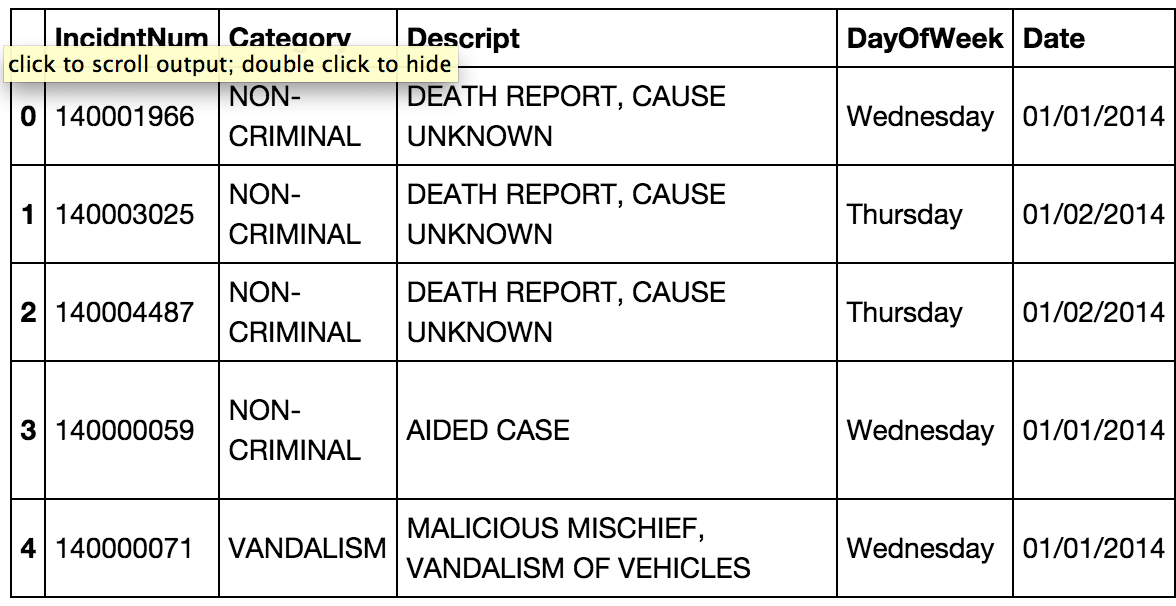
\includegraphics[scale=0.5]{sf_city_sample_1.png} \\
  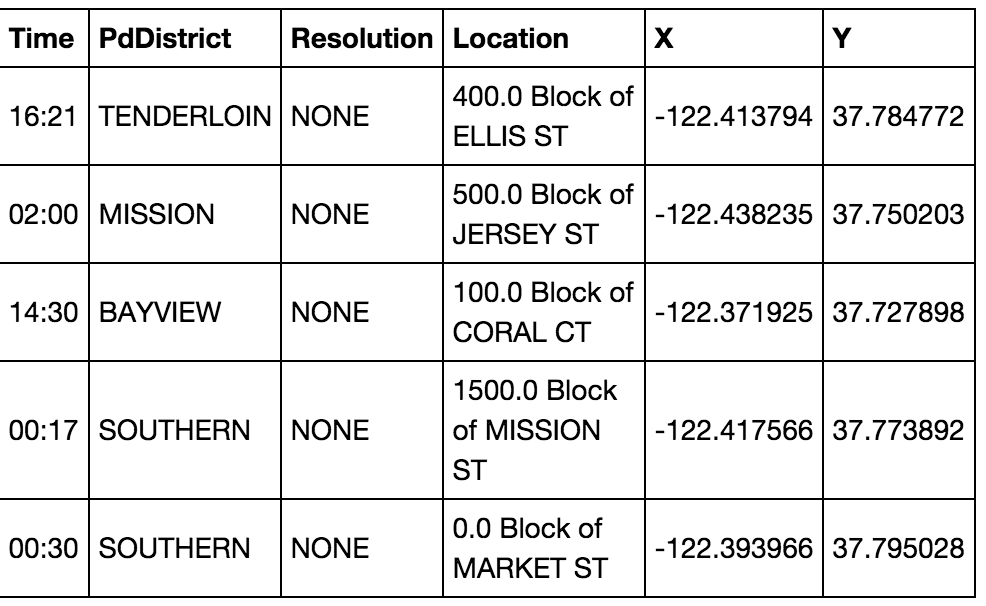
\includegraphics[scale=0.5]{sf_city_sample_2.png} \\
  Figure 1: Sample of San Francisco crime data set
\end{center}

The majority of the fields are self-explanatory. However, there are a few
things to note:
\begin{enumerate}
\item Category and descript are both categories, but category is more
  general. There are only 36 different ``Categories'' while there are 499
  different ``Descript''s in the year of 2014.
\item Resolution, though none are shown in the sample above, denote whether
  any action was taken and what that action was.
\item X denotes longitude, while Y denote latitude.
\end{enumerate}

A more detailed analysis is in the attached \texttt{analysis.ipynb}.

\subsection{Yelp Data Set}

Yelp.com is a platform which publishes crowd-sourced reviews about local
businesses. On Yelp, customers who have used the services of local
businesses may write reviews of these businesses and provide ratings of
their satisfaction. Reviewers may select from between 1 to 5 stars for each
review they make, and a business's average rating is the average of the
ratings of each of the reviews it has received. Yelp supplies a platform
for all kinds of local businesses ranging from restaurants to barbers to
museums; however, for the purpose of our research, we will look primarily
at restaurants as they are a very large majority of the reviews on Yelp.

There are two primary ways to access the data on Yelp. First, we can
utilize the search / business API
(\url{http://www.yelp.com/developers/documentation}). The API provides a
way to search for local businesses matching a particular key term
(``restaurants'', for example) near a geographical location, and get all
the rating / review information about that restaurant. The API further
allows us to narrow the search to only the geographically closest
restaurants (not ranked by rating). This gives us a way to link the
geographical location of crime incidents to the types of restaurants near
that incident.

The other way of accessing Yelp data is through the academic data set
(\url{https://www.yelp.com/academic_dataset}). The Yelp academic data set
provides all the data and associated reviews of the 250 closest businesses
to each of 30 universities, including UC Berkeley. Although not a random
sample of all businesses on Yelp, the academic data set provides a much
better estimate of all businesses in the Yelp data set population. For the
purposes of the analysis, we will assume for now that this data set is
a perfect sample of the entire Yelp data set, and that its average is
indicative of the Yelp-wide average. Issues with this assumption will be
addressed in the \textbf{\nameref{sec:lessons-learned}} section.

\section{Methods}
\label{sec:methods}

\subsection{Data Fetching}

The bulk of our work was done in trying to get data from Yelp. As
mentioned, there were two main ways that Yelp provides to access data, and
those are the API and the academic data set.

To access the Yelp API, Yelp provided sample Python code
(\url{https://github.com/Yelp/yelp-api/tree/master/v2/python}). However, as
we found out, the sample code was buggy -- not only did the code fail on
certain calls, it even failed on the default call when the search term was
``dinner'' and the location was ``San Francisco, CA''. We contacted Yelp
API support about this issue, but it seemed that the API wasn't
well-maintained, and Yelp engineers didn't have time to update or fix the
sample code. Therefore, we decided to fix the bug ourselves.

After much investigation, we figured out that whereas Python's
\texttt{urllib} library encoded spaces into ``+'' characters, Yelp's
server-side authentication expected the OAuth-signed URLs to use ``\%20''
as the proper encoding for space. In this context (the query arguments in a
URL), both should be valid, but Yelp's authenticator only expected the
latter. After figuring this out, we let the Yelp engineers know of the bug,
and were able to build a temporary work-around to fetch our data.

We also encountered other problems in data fetching. In addition to the
bugs in the API, there were rate limiting and quantity limiting issues as
well. In particular, we could only access 20 results at a time, and a
maximum of 40 total results for searches that sorted the results by only
distance or rating. With searches not by distance or rating, Yelp enforced
its own ranking to its results. Results further down the results page
became so varied that they no longer matched the keyword (for example, Yep
may provide a gym even though ``food'' was specified simply because the gym
was much closer than any other ``food'' locations). All of the above
limited the ways in which we could obtain and analyze Yelp data.

For us, the ideal way to get Yelp data would be to have a data set
containing data on every single restaurant in San Francisco. This would
have been the most ideal solution as
\begin{enumerate}
\item we could then compare the \textit{properties of restaurants} near
  crimes to the general population of restaurants in San Francisco
  properly. The way we do this instead is to use the academic data set, but
  that includes data from other cities
\item the data we had would be the \textit{entire population} of restaurants in San
  Francisco (that Yelp has in their database)
\item we could then compare any other \textit{location-based data} (like
  population density) and determine any confounding factors in our
  statistical model. This wasn't discovered until after our t-test
  results. The way we had to access the data instead introduced bias
  towards high-crime areas into the data set.
\end{enumerate}

Further, we weren't able to get as much data as we needed (because of
Yelp's rate limiting). However, it was still possible to search for the
closest restaurants near any location specified by longitude and
latitude. As a result, we decided to search for the 20 closest restaurants
near each crime and look at the characteristics of this set of restaurants.

In the end, we were able to build a fault-tolerant work-around to Yelp's
broken authentication system. We queried Yelp's API for the 20 closest
restaurants near each crime in the City of San Francisco crime data set for
a total of 12,000 crimes (9704 unique incidents due to multiple criminal
offenses per incident). These results were stored in the MongoDB instance
that we installed on our EC2 server.

\subsection{Visualization}

After fetching the data, % TODO

To create the heatmap for crime density, we took the map and created a 100
x 100 grid where we assigned a value to each spot on the grid based on the
amount of crimes in the area. We used the numpy module gaussian\_kde to help
us accomplish this. Then we exported this data structure as a csv with
fields longitude, latitude, and density. Then using heatmap.js, a
javascript library, we were able to create a heatmap layer over the Google
map, which we got using the Google maps API, of the region.

To create the plot of the yelp data, we had to first get our data in a csv
file with the fields longitude, latitude, and density. Once these fields
were found, we used the d3 library in javascript to plot circles on a
Google map based on their rating with red being every data point in the
95th percentile, yellow 75th percentile, green 50th percentile, and
elsewhere blue.

Lastly to create the last plot of the near crime data, the method was very
similar to the plot of all the Yelp ratings, except that the amount of data
was less and the gradient was slightly different being: ratings > 4.5 :
black, ratings = 4.5: red, ratings >=4: gold, ratings >=3.5: green, other:
blue.

\subsection{Looking for Correlations}

Our primary purpose (initially) was to determine how crime affected
restaurant ratings. Specifically, given the limitations of the data we
could get from Yelp, we wanted to see whether Yelp restaurant ratings were
any different when they were near crime hotspots.

At this point, we could access two data sets -- the data set of
``near-crime'' restaurants, obtained through querying for restaurants near
crime incident locations via the Yelp API, and the Yelp academic data
set. Given this data, we had a few options to draw a correlation:
\begin{enumerate}
\item We could look at the ``average rating'' of a crime -- that is, we
  could take the average rating of the 20 closest restaurants to a crime
  incident and call that the average rating of restaurants near that
  crime. Then, we could compare that rating with the Yelp-wide average from
  the academic data set.
\item We could look at all the \textit{restaurants} near any of the crime
  incidents in the crime data set. Then, we can put these together as a set
  of ``near-crime'' restaurants, and look at the rating distribution of
  these compared to the academic data set.
\end{enumerate}
We had originally planned to execute option 1. However, as we realized from
exploring the crime data set, crime density is very different for different
areas of San Francisco. If we look at the average rating of each crime, it
is likely that the results would be very heavily weighted by the ratings of
restaurants in high crime density areas (ie. Market Street). Although our
very purpose was to show that high crime density areas were prone to
different kinds of Yelp ratings, we did not want to artificially induce
this by weighting the results by the crime density itself. Therefore, we
chose the second option. Surprisingly, we discovered that in the 9704
unique incidents we looked at and the 194080 restaurants near those
incidents, there were only a total of 658 unique restaurants. This implies
that the crimes were indeed very clustered, and that use of the ``average
rating of a crime'' method (option 1) would have resulted in significant
bias to restaurants near the clustered areas. A further examination of the
visualizations indicate that crime was indeed highly clustered near Market
Street. This will be discussed more in the \textbf{\nameref{sec:results}}
section.

To determine whether there were any significant differences between the two
data sets, we used a Student's t-test as our statistical hypothesis
test. In this case, the null hypothesis was that the two data sets, both of
Yelp ratings in San Francisco, have identical expected values (means). The
t-test results are more thoroughly discussed in the
\textbf{\nameref{sec:results}} section. Through the analysis, however, we
learned instead that restaurants near high-crime areas actually had higher
ratings than the Yelp-wide average. This indicates that our hypothesis was
wrong. However, we also realized around this time that any correlation,
positive or negative, does not imply causation.

\subsection{Accounting for Population Density}

In an effort to learn why our hypothesis was wrong, we began considering
confounding factors. The two heatmaps we created seem to indicate that
population density was key.

% TODO snapshot of the data?


To gather the data on population density, we found a database file (.dbf)
from \url{data.sfgov.org} that contained a table that mapped tract (a unit
of area used by the census) to population density. We were also able to
find another data set that contained the tract centers (longitude and
latitude) for each tract. By associating each longitude and latitude pair
with the closest tract center (using great-circle distance for the Earth),
and then joining the population-density-by-tract-table on tract, we could
estimate which tract each restaurant or crime was in, and find an
associated population density for a restaurant or crime. The result allowed
us to look for a possible correlation between crime density and population
density.
\begin{center}
  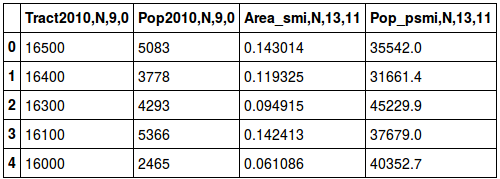
\includegraphics[scale=0.5]{raw_popdensitydata.png} \\
  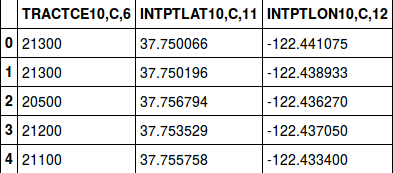
\includegraphics[scale=0.5]{tract_raw_data.png} \\
  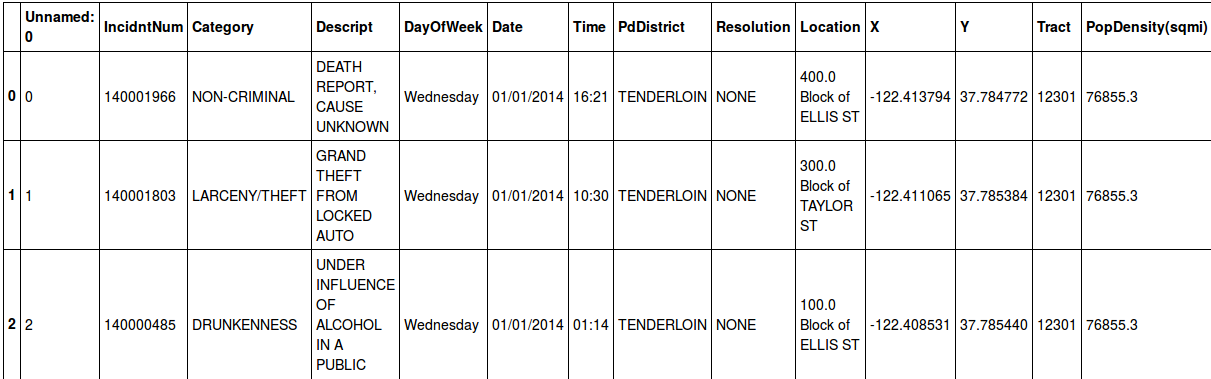
\includegraphics[scale=0.5]{full_population_density.png} \\

  Figure 1: Screen shots of population density data and tract data as well as final joined table of crime and population density
\end{center}

One difficulty we had with integrating this data was that the data was
given to us divided up into tracts, which are standardized regions of land
used by the government to collect census data. However, the crime data, and
therefore the Yelp data, were based on specific latitude and longitude
coordinates. A better way to have done it would have been to look at crimes
density by tract as well as average yelp data by tract. This would have
possibly allowed us to draw correlations with more conviction as well as
allow us to implement other statistical tools such as a regression. Alas,
we happened to collect the crime and Yelp data before the population
density, and it would have been too time consuming to recollect all the
crime density and Yelp ratings.

\section{Tools}

\begin{itemize}
\item pandas -- Pandas was our primary means of manipulating data sets. We
  used Pandas in our data fetching, data cleaning, and data analysis
  process.
\item MongoDB -- We installed MongoDB on the EC2 server and used it
  primarily for storing Yelp data. MongoDB was a great choice because the
  document-based nature of MongoDB was perfect for storing all the JSON
  documents we received from the Yelp API. In addition, we weren't sure
  what kind of data we needed to store when we first began fetching data,
  so using Mongo allowed us to easily keep all of the data in case we
  needed more than what we had thought.
\item pyMongo -- pyMongo was our choice Python interface to MongoDB.
\item numpy -- NumPy was used in conjunction with both Pandas and SciPy.
\item scipy -- We used SciPy mostly for its large library of statistical
  methods (t-tests, etc.).
\item D3.js -- We used D3 in conjunction with other frameworks when
  visualizing the data.
\item Google Maps API -- The Google Maps API provided a base for many of
  the location-based visualizations we needed to create. In addition, the
  Google Maps API also had a heatmap plugin, which we tried in addition to
  heatmap.js.
\item heatmap.js -- We primarily used heatmap.js for our heatmap
  visualizations.
\end{itemize}

\section{Results}
\label{sec:results}

A preliminary analysis of just the public safety data set is available in
the attached \texttt{analysis.pynb}. Below follows our results and
conclusions from looking at Yelp restaurant rating data near crime
hotspots.

\subsection{Visualizations}

\begin{center}
  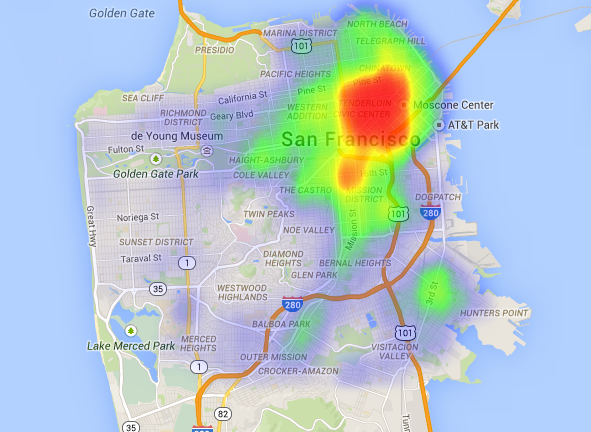
\includegraphics[keepaspectratio=true, width=350px]{crime_density_heatmap.png}
  Figure 2: Heatmap of crime density \\[20pt]

  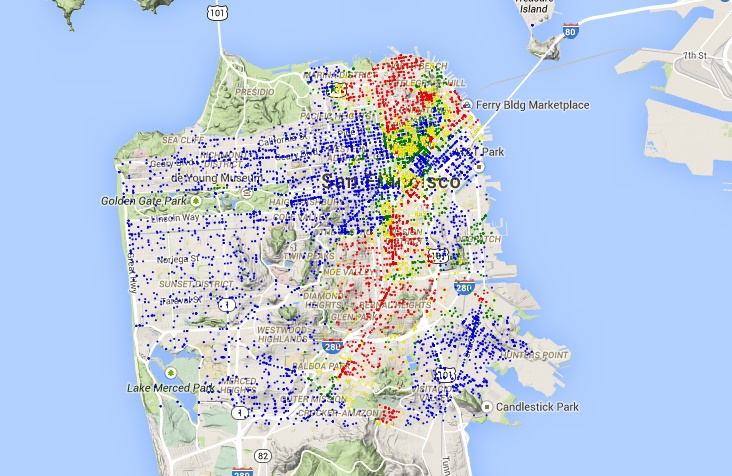
\includegraphics[keepaspectratio=true, width=350px]{all_yelp_ratings_plotted.jpg}
  Figure 3: Plot of ``average Yelp rating of crimes''. Each point
  corresponds to a crime, and the color corresponds to the average rating
  of the closest 20 restaurants to that crime. \\[20pt]

  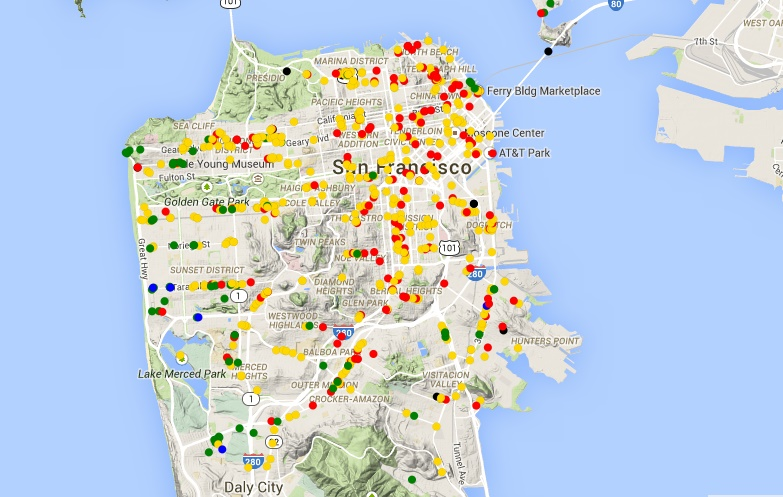
\includegraphics[keepaspectratio=true, width=350px]{unique_yelp_rating_plot.jpg}
  Figure 5: Plot of Yelp ratings for restaurants in the near-crime data
  set. Black = 5.0; red = 4.5; yellow = 4.0; green = 3.5; blue = 3.0 \\[20pt]
\end{center}

\subsection{Putting it together}

The results of the t-test between the near-crime data set and subsets of
the academic data set are detailed in Table 1.

\begin{center}
  \begin{tabular}{ | l | c | c | c | c | }
    \hline
    Data set                       & Mean  & Std   & t-statistic* & p-value*    \\
    \hline
    Near-crime                     & 4.072 & 0.327 &              &             \\
    All businesses (all)           & 3.618 & 0.933 & -12.441      & 2.39\e{-35} \\
    All businesses (Berkeley)      & 3.629 & 0.837 & -12.390      & 3.43\e{-33} \\
    All businesses (Stanford)      & 3.696 & 0.846 & -8.310       & 4.34\e{-16} \\
    All businesses (Los Angeles)   & 3.571 & 0.988 & -12.542      & 1.66\e{-34} \\
    Restaurants only (all)         & 3.482 & 0.739 & -20.291      & 7.10\e{-89} \\
    Restaurants only (Berkeley)    & 3.413 & 0.618 & -20.490      & 9.34\e{-77} \\
    Restaurants only (Stanford)    & 3.307 & 0.520 & -14.367      & 3.30\e{-41} \\
    Restaurants only (Los Angeles) & 3.431 & 0.773 & -18.797      & 2.28\e{-68} \\
    \hline
  \end{tabular}

  Table 1: t-test results against ``near-crime'' data set
\end{center}
* against the ``near-crime'' data set

The ``all businesses'' data sets refer to all the businesses provided by
the academic data set, whereas the ``restaurants only'' data sets filtered
out only the businesses in the academic data set that had ``Food'' or
``Restaurants'' as one of the items in its category field.

From the p-values of each t-test it is clear that the null hypothesis can
be rejected, and that the ``near-crime'' data set does not have the same
average Yelp rating as the other data sets. The following two plots provide
a better picture of the actual distribution of each data set.

\begin{center}
  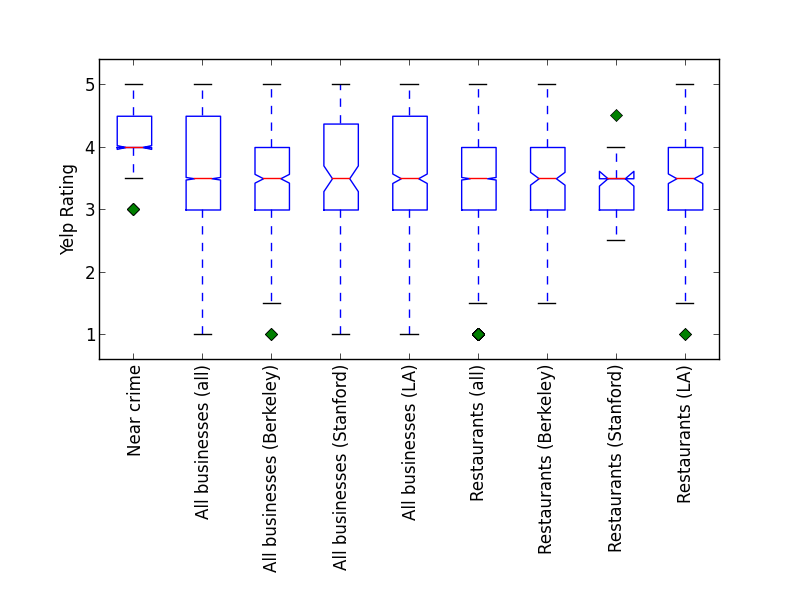
\includegraphics[keepaspectratio=true, width=320px]{boxplot.png}
  Figure 2: Box-and-whiskers plot of distribution of the ratings of
  different data sets \\[20pt]

  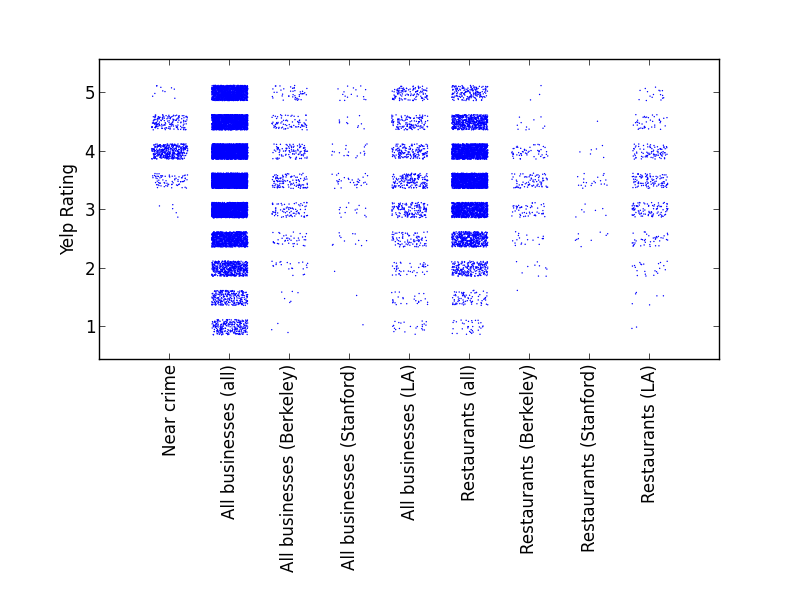
\includegraphics[keepaspectratio=true, width=320px]{scatter_plot.png}
  Figure 3: Scatter plot of distribution of the ratings of different data
  sets. Points plotted with certain randomness to show distribution of
  points. \\[20pt]
\end{center}

However, the data indicates that our initial hypothesis was also wrong --
we found instead that the restaurants near crimes were actually
\textit{higher} rated than the general population of restaurants. To us,
this was extremely counterintuitive. Our original hypothesis was that crime
would negatively affect restaurant ratings. However, the data seems to show
that crime was instead positively correlated with ratings. As we were
looking for explanations, we also realized that the tests we have been
doing would not prove causation anyways. It's possible that crime
positively affects restaurant ratings, or that restaurant ratings increase
the crime rate, but it's also possible that both are correlated with a
third confounding factor. In particular, from the visualizations we created
earlier, it's very likely that population density would be a factor. Areas
near Market Street are known to be the most popular areas in San Francisco,
for work, shopping, and many other things. A high population density would
spark growth and increase competition, so any restaurants that are able to
stay in the area must be high quality. A high population density would also
attract crime, as there are more targets, and the chaos of the busy streets
may make it easier to get away. As we were not familiar with these
statistical notions when we formulated our problem statement, we had not
thought of problems like these when we started.

Due to the limitations of the Yelp API, we could not get Yelp data with an
even distribution across all of San Francisco. Given what we had, we wanted
to compare the population density of the areas of near-crime restaurants to
the population density of the restaurants in the other sets. However,
because our academic data set had restaurants all across the United States
where we didn't have ready access to population density data, it was
impossible to calculate population density for these areas. Further,
population varies more by city than areas within the city, so variations in
those restaurants are not telling at all.

The best alternative was to instead compare the population density of the
areas of near-crime restaurants to the total population density of San
Francisco. Although the results of this test would not be directly related
to the test performed above, it would provide exploratory insight into the
reason behind why our hypothesis was wrong.

Using the methods described in the \textbf{\nameref{sec:methods}} section,
we decided to also compare the population density of those areas.

\subsection{Population Density}

Another simpler t-test was performed in order to see how high-crime areas
were correlated with population density. From the population density data,
we found that the total population density of the city of San Francisco was
17143.59 people per square mile. We conducted a one-sample t-test to
determine whether either of the following two data sets were significantly
different from the city of San Francisco mean population density. The first
data set is that of the population density of the near-crime restaurant
data set. That is, it is the population densities of tracts containing the
Yelp restaurants which were found to be close to crime incidents. The next
is the data set of the population density of crime itself. In other words,
it is the population densities of the tracts of 9704 distinct crimes. We
will call the first one the ``restaurants'' data set and the second one the
``crimes'' data set.

\begin{center}
  \begin{tabular}{ | l | c | c | c | c | }
    \hline
    Data set    & Mean     & Std      & t-statistic* & p-value*      \\
    \hline
    Restaurants & 25437.36 & 15694.58 & 13.56        & 4.34\e{-37}   \\
    Crimes      & 34488.61 & 30239.04 & 62.83        & $\approx$ 0.0 \\
    \hline
  \end{tabular}

  Table 2: t-test results against known population density mean
\end{center}
* against known population density mean of 17143.59 people per square mile

The results indicate that the restaurants and crimes were indeed correlated
with a significantly higher population density. This confirms our suspicion
that population density, or another similar confounding factor, played a
role in the correlation between crime density and Yelp ratings. However,
again, as we lack the data and tools to prove this definitively, we can
only say that further investigation into the relationships between crime
density, Yelp rating distribution, and population density would be a
profitable cause.

\section{Lessons Learned}
\label{sec:lessons-learned}

Our project was nowhere near perfect, but through our project, we learned
many, many valuable lessons that will no doubt benefit any future data
science projects we perform.

\subsection{The Problem Statement}

Perhaps the most important thing that we learned is to formulate a clear
problem statement from the very beginning. When we began the project, we
were looking to find interesting correlations between Yelp restaurant
ratings and crime occurrences. However, as we didn't have experience with
data science projects, we weren't used to formulating rigorous statistical
hypotheses. As a result, we forgot about the fact that correlation did not
imply causation. Furthermore, we did not think through what data we can
access, how to combine the data together, and other confounding factors in
our model. If we had thought clearly through our entire problem statement
and formulated a plan of attack, then given the limitation of the Yelp API,
we might have changed our project to be geared towards other APIs or data
sets that could give us a picture of the entirety of San Francisco.

\subsection{Let the Data Speak}

Having a clear problem statement, however, does not mean assuming a certain
hypothesis before we see the data. In this project, we realized that we had
held our hypothesis as fact throughout the course of most of our
investigation. A lot of our plans to visualize the data, for example, were
made before we even looked at the data, and they were made to show that a
correlation did indeed exist. On a similar note, if we could had tried to
get the data and conduct the tests of significance first, we would have
realized the problem with correlations vs. causation earlier on, and that
would have given us more leeway in planning our next steps.

\subsection{The Yelp API}

The Yelp API was a huge problem for us in this project. There were multiple
issues with it. First, and most importantly, was that we couldn't get a
evenly distributed sample of restaurants in San Francisco. Ideally, we
would be able to get the entire data set of all restaurants in San
Francisco, but even if that was not possible, an truly random sample of the
restaurants in San Francisco would have been much nicer. If we had this
data, we would then be able to correlate restaurants with location without
any bias, and then we could use any location-based data in our model (such
as population density). The way we were forced to access data meant that we
were only able to find restaurants that were near crimes in the first
place. This makes our data set inherently biased. Given this bias, we were
only able to analyze the data in a particular way (compare near-crime
restaurants vs. the general population of restaurants).

Because of this limitation, we had to use the academic data set as a
representative sample of the entire Yelp restaurant population. Because the
academic data set was of restaurants outside of San Francisco, this posed
two major problems:
\begin{enumerate}
\item All the data we obtained for other purposes do not pertain to the
  academic data set. Because of this, we could only use the academic data
  set in a separate analysis from all the other data with which we were
  working.
\item The academic data set is not necessarily a representative sample of
  the entire Yelp restaurant population. For one thing, it's just a sample
  of the closest 250 businesses to certain universities. Aside from the
  fact that businesses near universities themselves may be biased, the fact
  that the data set spans different cities may be bias in itself. San
  Francisco's restaurant rating distribution may vary highly from those of
  Berkeley, Stanford, Los Angeles etc.
\end{enumerate}

Furthermore, we also had technical issues with the Yelp API. We had found
many bugs in the Yelp API and sample code, both of which were no longer
maintained. Aside from the authentication bug mentioned, the Yelp API also
had issues handling Unicode. The rate limiting and the slow response rate
of the Yelp API also meant that we couldn't query every single location in
San Francisco to obtain data for every single restaurant in Yelp's
database. Data fetching was tedious and marginally better than scraping at
best. Furthermore, the API lacked some of the properties displayed on the
website such as price range (denoted by a number of dollar signs from 1 to
4). Characteristics like this may have been better correlated with crime
density, or would at least have given us a clearer picture of the reason
behind why our hypothesis was wrong. Keyword search with location was also
a strange idea, because due to the way search is implemented there are
necessarily restaurants that may not be included in a search result (false
negatives in the search). Usually, for the purposes of a human user, this
would not be a problem, but if the search filters out actual restaurants
because it doesn't match the keyword as well, then this process introduces
bias into our data. Finally, in hindsight, Yelp rating data was too limited
to be informative. The API only provides rating data accurate to 0.5
increments, so there are only a total of 10 different ratings a restaurant
could have. We had asked Yelp developers through email to provide us with a
separate data set with more resolution in ratings, but they weren't able to
provide us with anything.

\subsection{Causation}

As mentioned above, our biggest problem by the end of the project was that,
given the data we could access and the limitations we had, we weren't able
to show causation or lack thereof. This is partly because we didn't have a
clear problem statement to begin with, but is also because we didn't have
the statistical background to think rigorously about the process by which
we do data science, and the implications of finding a correlation. We also
didn't realize that confounding factors were something that almost
definitely had to account for, as our original plan was just to predict
crime density using restaurant ratings by utilizing machine learning.

-- unfortunately couldn't show causation but good idea of why

\bibliographystyle{IEEEtran}
\bibliography{writeup-bibliography}

\end{document}
